\begin{blocksection}
\question
\textbf{recurses}\\
Fill in each blank in the code below so that its environment diagram is the following.\\
You are not allowed to use operations like +, -, *, /, \%, \lstinline{max}, and \lstinline{min}.

\begin{multicols}{2}
\begin{lstlisting}
a = [0]
def recurses(x):
    if x == 0:
        return _______________
    elif type(x) == int:
        a[0] += x
        return _______________
    else:
        return ______________\
        ______________________
recurses(lambda x: x * x)
\end{lstlisting}


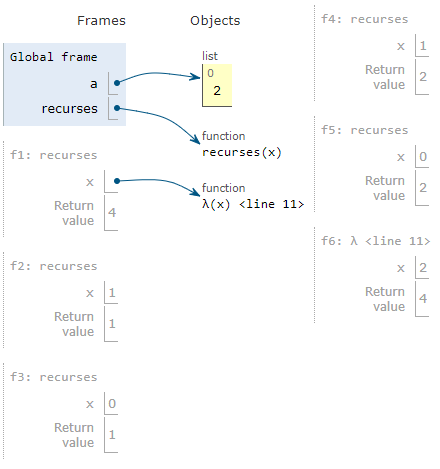
\includegraphics[width=\linewidth]{recurses.png}
\end{multicols}
\end{blocksection}

\begin{solution}[2in]
\begin{blocksection}
\textbf{Solution}
\begin{lstlisting}
a = [0]
def recurses(x):
    if x == 0:
        return a[0]
    elif type(x) == int:
        a[0] += x
        return recurses(0)
    else:
        return x(recurses(recurses(1)))
recurses(lambda x: x * x)
\end{lstlisting}
\end{blocksection}
\end{solution}

\begin{guide}
\begin{blocksection}
\vspace{5mm}
\textbf{Teaching Tips}
\begin{itemize}
\item This problem is difficult! Students may need hints to get started.
\item The easiest line to solve is the first blank, the base case. What does the environment diagram show is returned when \lstinline{x == 0}?
\begin{itemize}
\item This value changes, so how can we return a changing value in one line?
\item With a variable! In this case, the only other variable is \lstinline{a[0]}.
\end{itemize}
\item To figure out what the second blank is, observe the frames after frames of \lstinline{recurses} where \lstinline{x} is a number != 0.
\item You can observe that in both cases, the next frame is a \lstinline{recurses} where \lstinline{x = 0}, so it follows that the answer is \lstinline{recurses(0)}.
\item The last line is the trickiest, and it may be good to let students ponder it for a few minutes.
\item It may be easiest to work from the inside \lstinline{recurses} call to the outside $\lambda$ call.
\item Draw out which frames are created with each function call until you have successfully replicated the environment diagram!
\end{itemize}
\end{blocksection}
\end{guide}
